\documentclass[tikz,border=8pt]{standalone}
\usepackage[utf8]{inputenc}
\usepackage[OT4,plmath]{polski}
\usepackage{amsmath}
\begin{document}
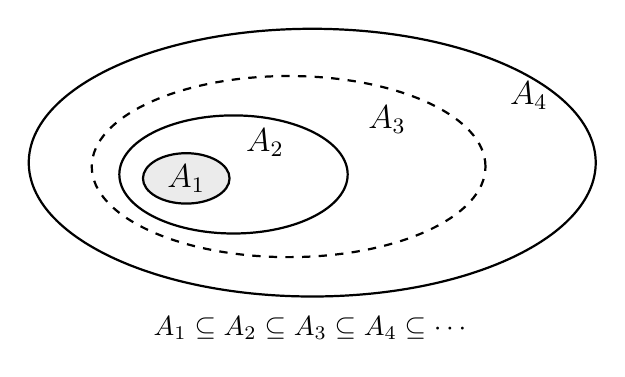
\begin{tikzpicture}[font=\large]
  \draw[thick] (0,0) ellipse (3.6cm and 1.7cm);
  \draw[thick,dashed] (-.3,-.05) ellipse (2.5cm and 1.15cm);
  \draw[thick] (-1,-.15) ellipse (1.45cm and .75cm);
  \draw[thick,fill=black!8] (-1.6,-.2) ellipse (.55cm and .32cm);
  \node at (-1.6,-.2) {$A_1$};
  \node at (-.6,.25) {$A_2$};
  \node at (.95,.55) {$A_3$};
  \node at (2.75,.85) {$A_4$};
  \node[font=\normalsize] at (0,-2.1)
    {$A_1\subseteq A_2\subseteq A_3\subseteq A_4\subseteq\cdots$};
\end{tikzpicture}
\end{document}
